\documentclass[11pt,class=report,crop=false]{standalone}
\usepackage{exo7hilisit}

\begin{document}


\entete{Hilisit}{Capacité mathématiques}

\titre{Exercices -- \'Equations différentielles}

\bigskip
\bigskip


%%%%%%%%%%%%%%%%%%%%%%%%%%%%%%%%%%%%%%%%%%%%%%%%%%%%%%%%%%%%
\section{Primitive}

\exercice{}
\enonce
Mettre en correspondance chaque fonction $f$ avec une de ses primitives $F$. 
 \begin{itemize}
  \item $f_1(x) = -6\sin(2x)$, $f_2(x) = 2x$, $f_3(x) = (x+1)e^x$, $f_4(x) = -6\sin(3x)$, $f_5(x) = 2xe^{x^2}$, $f_6(x)=2x+2$.
  \item $F_a(x) = 2\cos(3x)$, $F_b(x) = 3\cos(2x)$, $F_c(x) = (x+1)^2$, $F_d(x) = x^2+1$, $F_e(x) = e^{x^2}$, $F_f(x) = xe^x$. 
\end{itemize} 
\finenonce

\indication
$F$ est une primitive de $f$ si $F'(x)=f(x)$ (pour tout $x$ de l'ensemble de définition).
\finindication

\correction
\sauteligne
\begin{enumerate}
  \item $F_a(x) = 2\cos(3x)$, $F_a'(x) = f_4(x) = -6\sin(3x)$.
  \item $F_b(x) = 3\cos(2x)$, $F_b'(x) = f_1(x) = -6\sin(2x)$.
  \item $F_c(x) = (x+1)^2$, $F_c'(x) = f_6(x) = 2x+2$.
  \item $F_d(x) = x^2+1$, $F_d'(x) = f_2(x) = 2x$.
  \item $F_e(x) = e^{x^2}$, $F_e'(x) = f_5(x) = 2xe^{x^2}$.
  \item $F_f(x) = xe^x$, $F_f'(x) = f_3(x) = (x+1)e^x$.
\end{enumerate}
\fincorrection
\finexercice


\exercice{}
\enonce
Pour chacune des fonctions $f$ suivantes, déterminer une primitive $F$.
\begin{enumerate}
  \item $f_1(x) = -\cos(2x)$
  \item $f_2(x) = x^3-7x^2+1$
  \item $f_3(x) = \frac{1}{2x-1}$ (sur $]-\frac12,+\infty[$)
  \item $f_4(x) = e^{\pi x-3}$
  \item $f_5(x) = -(x-2)^2$
  \item $f_6(x) = \sin(8(x+1))$
\end{enumerate} 
\finenonce

\indication
Il s'agit de trouver une fonction $F$ telle que $F'(x) = f(x)$. Il faut bien connaître ses formules des dérivées usuelles.
\finindication

\correction
\sauteligne
\begin{enumerate}
  \item $F_1(x) = -\frac12\sin(2x)$, on vérifie que $F_1'(x) = f_1(x)$.
  \item $F_2(x) = \frac14x^4-\frac73x^3+x$, car une primitive de $x^k$ est $\frac{1}{k+1}x^{x+1}$ (pour $k \ne -1$).
  \item $F_3(x) = \frac12\ln(2x-1)$ car $(\ln(u))' = \frac{u'}{u}$ avec ici $u(x)=2x-1$.
  \item $F_4(x) = \frac{1}{\pi}e^{\pi x-3}$ car $(e^u)' = u'e^u$ avec ici $u(x)=\pi x-3$.
  \item $F_5(x) = -\frac{x^3}{3}+2x^2-4x$ car $f_5(x) = -x^2+4x-4$. On peut aussi écrire $F_5(x) = -\frac13(x-2)^3$. 
  \item $F_6(x) = -\frac18\cos(8(x+1))$ car $(\cos(u))' = -u' \sin(u)$.
\end{enumerate}
Dans tous les cas, si $F$ est une primitive, alors pour toute constante $C$, $F+C$ est aussi une primitive.
\fincorrection
\finexercice


\exercice{}
\enonce
\sauteligne
\begin{enumerate}
  \item 
  \begin{enumerate}
    \item Quelle est la dérivée de la fonction $x \mapsto u^k(x)$ où $x \mapsto u(x)$ est une fonction et $k$ un entier ?
    \item Calculer les dérivées des fonctions définies par $(x^4+7x^3+2)^3$, $\cos^3(2x)$, $\ln^2(x)$, $\frac{1}{(x^2+1)^2}$.
    \item Déterminer une primitive des fonctions définies par $x(x^2+5)^5$, $\sin(x) \cos^3(x)$, $\frac{\ln^n(x)}{x}$ (où $n\ge0$).
  \end{enumerate} 

  \item 
  \begin{enumerate}
    \item Quelle est la dérivée de la fonction $x \mapsto e^{u(x)}$ où $x \mapsto u(x)$ est une fonction ?
    \item Calculer les dérivées des fonctions définies par $e^{-5x}$, $e^{x^3-2x}$, $e^{\sin(3x)}$, $e^{1/x}$.
    \item Déterminer une primitive des fonctions définies par $e^{8x+1}$, $xe^{x^2+1}$, $\frac{e^{\sqrt x}}{\sqrt x}$.
  \end{enumerate} 


  \item 
  \begin{enumerate}
    \item Quelle est la dérivée de la fonction $x \mapsto \ln(u(x))$ où $x \mapsto u(x)$ est une fonction strictement positive ?
    \item Calculer les dérivées des fonctions définies par $\ln(x^3-2)$, $\ln(e^x+e^{-x})$, $\ln(1/x)$, $\ln(\cos(x^2))$.
    \item Déterminer une primitive des fonctions définies par $\frac{1}{x+4}$ (sur $]-4,+\infty[$), $\frac{x}{x^2+4}$ (sur $\Rr$), $\frac{\cos(x)}{\sin(x)}$ (pour les $x$ où $\sin(x)>0$).
  \end{enumerate} 

\end{enumerate} 
\finenonce

\indication
La dérivée d'une composition $f(u(x))$ est $u'(x) f'(u(x))$.
Pour déterminer les primitives il faut reconnaître la fonction sous une forme $u'(x) f'(u(x))$, afin de déterminer qu'une primitive est $f(u(x))$.
\finindication

\correction
\sauteligne
\begin{enumerate}
  \item 
  \begin{enumerate}
    \item La dérivée de $u^k(x)$ est $ku'(x)u^{k-1}(x)$.
    \item 
    \begin{itemize}
      \item La dérivée de $(x^4+7x^3+2)^3$ est $3(4x^3+21x^2)(x^4+7x^3+2)^2$.
      \item La dérivée de $\cos^3(2x)$ est $-6\sin(2x)\cos^2(2x)$.
      \item La dérivée de $\ln^2(x)$ est $\frac2x\ln(x)$. 
      \item La dérivée de $\frac{1}{(x^2+1)^2} = (x^2+1)^{-2}$ est $-2(2x)(x^2+1)^{-3}=\frac{-4x}{(x^2+1)^3}$.
    \end{itemize} 
    \item 
    \begin{itemize}
      \item Une primitive de $x(x^2+5)^5 = \frac1{12} \cdot 6 \cdot (2x) \cdot (x^2+5)^5$ est $\frac1{12} (x^2+5)^6$.
      \item Une primitive de $\sin(x) \cos^3(x)$ est $-\frac14\cos^4(x)$.
      \item Une primitive de $\frac{\ln^n(x)}{x}$ est $\frac{1}{n+1}\ln^{n+1}(x)$.
    \end{itemize} 
  \end{enumerate} 

  \item 
  \begin{enumerate}
    \item La dérivée de $e^{u(x)}$ est $u'(x)e^{u(x)}$.
    \item 
    \begin{itemize}
      \item La dérivée de $e^{-5x}$ est $-5e^{-5x}$.
      \item La dérivée de $e^{x^3-2x}$ est $(3x^2-2)e^{x^3-2x}$.
      \item La dérivée de $e^{\sin(3x)}$ est $3\cos(3x)e^{\sin(3x)}$.
      \item La dérivée de $e^{1/x}$ est $-\frac1{x^2}e^{1/x}$.
    \end{itemize} 

    \item 
    \begin{itemize}
      \item Une primitive de $e^{8x+1}$ est $\frac18e^{8x+1}$.
      \item Une primitive de $xe^{x^2+1}$ est $\frac12e^{x^2+1}$ 
      \item Une primitive de $\frac{e^{\sqrt x}}{\sqrt x}$ est $2e^{\sqrt x}$.
    \end{itemize} 
  \end{enumerate} 


  \item 
  \begin{enumerate}
    \item La dérivée de $\ln(u(x))$ est $\frac{u'(x)}{u(x)}$.
    \item 
    \begin{itemize}
      \item La dérivée de $\ln(x^3-2)$ est $\frac{3x^2}{x^3-2}$.
      \item La dérivée de $\ln(e^x+e^{-x})$ est $\frac{e^x-e^{-x}}{e^x+e^{-x}}$.
      \item La dérivée de $\ln(1/x)$ est $-\frac{1}{x}$ (c'est plus facile si on a remarqué que $\ln(1/x)=-\ln(x)$ !).
      \item La dérivée de $\ln(\cos(x^2))$ est $\frac{-2x\sin(x^2)}{\cos(x^2)}$.
    \end{itemize}

    \item 
    \begin{itemize}
      \item Une primitive de $\frac{1}{x+4}$ est $\ln(x+4)$.
      \item Une primitive de $\frac{x}{x^2+4}$ est $\frac12\ln(x^2+4)$.
      \item Une primitive de $\frac{\cos(x)}{\sin(x)}$ est $\ln(\sin(x))$.
    \end{itemize} 
  \end{enumerate} 

\end{enumerate} 
\fincorrection
\finexercice


\exercice{}
\enonce
\sauteligne
 \begin{enumerate}
  \item Pour la fonction $f$ représentée ci-dessous, déterminer quel est le graphe de la fonction $F_i$ qui correspond à une primitive de $f$.
\begin{center}
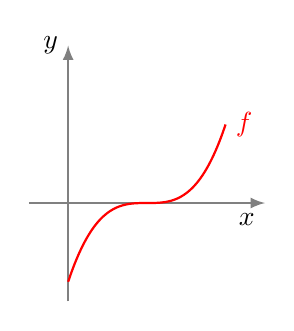
\begin{tikzpicture}[scale=1]
  \draw[->,>=latex,thick,gray] (-0.5,0) -- (2.5,0) node[below left,black] {$x$};
  \draw[->,>=latex,thick,gray] (0,-1.25) -- (0,2) node[left,black] {$y$};
  \draw[thick, color=red,domain=0:2, smooth,samples=50] plot (\x,{(\x-1)^3}) node[right]{$f$};
\end{tikzpicture}
\end{center}

\begin{center}
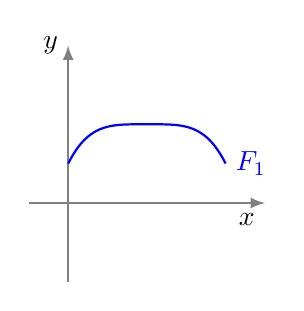
\begin{tikzpicture}[scale=1]
  \draw[->,>=latex,thick,gray] (-0.5,0) -- (2.5,0) node[below left,black] {$x$};
  \draw[->,>=latex,thick,gray] (0,-1) -- (0,2) node[left,black] {$y$};
  \draw[thick, color=blue,domain=0:2, smooth,samples=50] plot (\x,{-1/2*(\x-1)^4+1}) node[right]{$F_1$};
\end{tikzpicture}
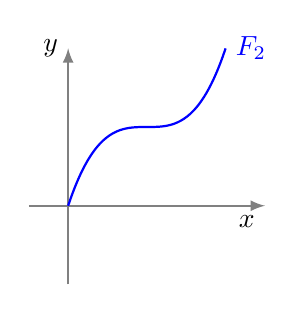
\begin{tikzpicture}[scale=1]
  \draw[->,>=latex,thick,gray] (-0.5,0) -- (2.5,0) node[below left,black] {$x$};
  \draw[->,>=latex,thick,gray] (0,-1) -- (0,2) node[left,black] {$y$};
  \draw[thick, color=blue,domain=0:2, smooth,samples=50] plot (\x,{(\x-1)^3+1}) node[right]{$F_2$};
\end{tikzpicture}
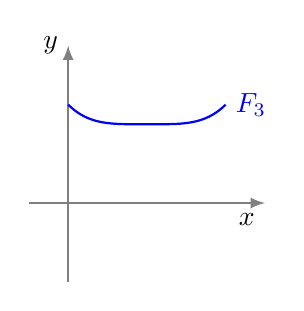
\begin{tikzpicture}[scale=1]
  \draw[->,>=latex,thick,gray] (-0.5,0) -- (2.5,0) node[below left,black] {$x$};
  \draw[->,>=latex,thick,gray] (0,-1) -- (0,2) node[left,black] {$y$};
  \draw[thick, color=blue,domain=0:2, smooth,samples=50] plot (\x,{1/4*(\x-1)^4+1}) node[right]{$F_3$};
\end{tikzpicture}
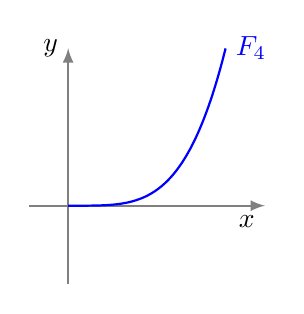
\begin{tikzpicture}[scale=1]
  \draw[->,>=latex,thick,gray] (-0.5,0) -- (2.5,0) node[below left,black] {$x$};
  \draw[->,>=latex,thick,gray] (0,-1) -- (0,2) node[left,black] {$y$};
  \draw[thick, color=blue,domain=0:2, smooth,samples=50] plot (\x,{1/8*\x^4}) node[right]{$F_4$};
\end{tikzpicture}
\end{center}

  \item Pour la fonction $f$ représentée ci-dessous, déterminer quel est le graphe de la fonction $F_i$ qui correspond à une primitive de $f$.
\begin{center}
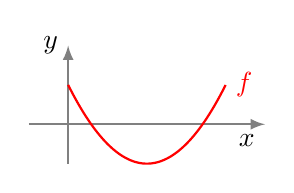
\begin{tikzpicture}[scale=1]
  \draw[->,>=latex,thick,gray] (-0.5,0) -- (2.5,0) node[below left,black] {$x$};
  \draw[->,>=latex,thick,gray] (0,-0.5) -- (0,1) node[left,black] {$y$};
  \draw[thick, color=red,domain=0:2, smooth,samples=50] plot (\x,{(\x-1)^2-1/2}) node[right]{$f$};
\end{tikzpicture}
\end{center}

\begin{center}
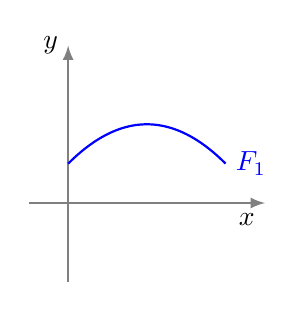
\begin{tikzpicture}[scale=1]
  \draw[->,>=latex,thick,gray] (-0.5,0) -- (2.5,0) node[below left,black] {$x$};
  \draw[->,>=latex,thick,gray] (0,-1) -- (0,2) node[left,black] {$y$};
  \draw[thick, color=blue,domain=0:2, smooth,samples=50] plot (\x,{-1/2*(\x-1)^2+1}) node[right]{$F_1$};
\end{tikzpicture}
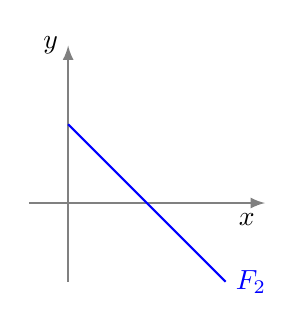
\begin{tikzpicture}[scale=1]
  \draw[->,>=latex,thick,gray] (-0.5,0) -- (2.5,0) node[below left,black] {$x$};
  \draw[->,>=latex,thick,gray] (0,-1) -- (0,2) node[left,black] {$y$};
  \draw[thick, color=blue,domain=0:2, smooth,samples=50] plot (\x,{-\x+1}) node[right]{$F_2$};
\end{tikzpicture}
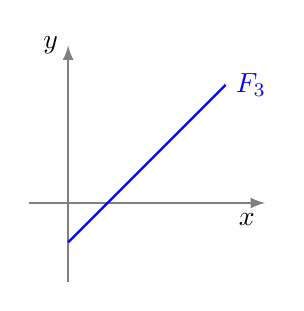
\begin{tikzpicture}[scale=1]
  \draw[->,>=latex,thick,gray] (-0.5,0) -- (2.5,0) node[below left,black] {$x$};
  \draw[->,>=latex,thick,gray] (0,-1) -- (0,2) node[left,black] {$y$};
  \draw[thick, color=blue,domain=0:2, smooth,samples=50] plot (\x,{\x-0.5}) node[right]{$F_3$};
\end{tikzpicture}
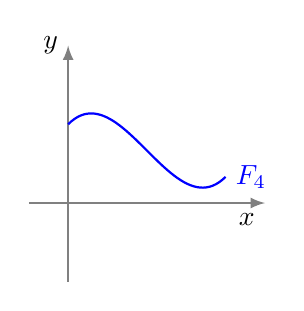
\begin{tikzpicture}[scale=1]
  \draw[->,>=latex,thick,gray] (-0.5,0) -- (2.5,0) node[below left,black] {$x$};
  \draw[->,>=latex,thick,gray] (0,-1) -- (0,2) node[left,black] {$y$};
  \draw[thick, color=blue,domain=0:2, smooth,samples=50] plot (\x,{2*(\x/2 - \x^2 + \x^3/3)+1}) node[right]{$F_4$};
\end{tikzpicture}
\end{center}

\end{enumerate} 
\finenonce

\indication
Il faut utiliser que la dérivée de $F$ est $f$ et utiliser le signe (et non pas la monotonie) de $f$ pour déterminer là où $F$ est croissante ou décroissante.
\finindication

\correction 
\sauteligne

Comme la dérivée de $F$ est $f$, là où $f$ est positive, $F$ est croissante ; là où $f$ est négative, $F$ est décroissante.
\begin{enumerate}
  \item $f = F'$ est négative puis positive : $F$ doit être d'abord décroissante, puis ensuite croissante. Ainsi il s'agit de $F_3$.
  \item $f = F'$ est positive, négative puis à nouveau positive. Donc $F$ est croissante, décroissante puis à nouveau croissante. Il s'agit de $F_4$.
\end{enumerate} 
\fincorrection
\finexercice


%%%%%%%%%%%%%%%%%%%%%%%%%%%%%%%%%%%%%%%%%%%%%%%%%%%%%%%%%%%%
\section{Notion d'équation différentielle}


\exercice{}
\enonce
Vérifier que les fonctions $f$ suivantes sont solutions de l'équation différentielle donnée.
\begin{enumerate}
  \item $f(x) = -e^{2x}$, $y'=2y$.
  \item $f(x) = \frac{1}{2-x}$, $y'=y^2$.
  \item $f(x) = (3+2x)e^x$, $y''-2y'+y=0$.
  \item $f(x) = Ce^{-x}+\sin(x)-\cos(x)$ (quelle que soit la constante $C$), $y'+y=2\sin(x)$
\end{enumerate} 
\finenonce

\indication
Il faut calculer la dérivée $f'(x)$ (et si besoin la dérivée seconde $f''(x)$) et vérifier que $f$ et $f'$ (et éventuellement $f''$) satisfont la relation donnée par l'équation différentielle (en remplaçant $y$ par $f$, $y'$ par $f'$...).
\finindication

\correction
\sauteligne
\begin{enumerate}
  \item $f(x) = -e^{2x}$, $f'(x) = -2e^{2x}$ donc on a bien $f'(x)=2f(x)$.
  \item $f(x) = \frac{1}{2-x}$, $f'(x) = \frac{1}{(2-x)^2}$ donc on a bien  $f'(x)=f(x)^2$.
  \item $f(x) = (3+2x)e^x$,  $f'(x) = (5+2x)e^x$, $f''(x) = (7+2x)e^x$ donc on a bien  $f''(x)-2f'(x)+f(x)=((3+2x) -2(5+2x)+(7+2x))e^x = 0\cdot e^x = 0$.
  \item $f(x) = Ce^{-x}+\sin(x)-\cos(x)$, $f'(x) = -Ce^{-x}+\cos(x)+\sin(x)$, donc on a bien  $f'(x)+f(x)=2\sin(x)$.
\end{enumerate} 
\fincorrection
\finexercice


\exercice{}
\enonce
Déterminer toutes les solutions constantes des équations différentielles suivantes.
\begin{enumerate}
  \item $y'+y=5$
  \item $y'=y^2-y$
  \item $y'=y^2-4y+1$
  \item $y' = y + x$
\end{enumerate} 
\finenonce

\indication
Si $f(x)=k$ est une fonction constante, alors $f'(x)=0$ pour tout $x$. Une des équations n'admet aucune solution constante !
\finindication

\correction
\sauteligne
 \begin{enumerate}
  \item Si $f$ est une fonction constante, alors $f(x)=k$ pour tout $x$, donc $f'(x)=0$ pour tout $x$. Si $f$ est solution de l'équation différentielle $y'+y=5$, alors $f'(x)+f(x)=5$ pour tout $x$, donc $0+k=5$, donc $k=5$. La seule solution constante est la solution $f(x)=5$ pour tout $x$.

  \item Si $f(x)=k$ est solution de l'équation différentielle $y'=y^2-y$, alors $f'(x)=f(x)^2-f(x)$ pour tout $x$, donc $0=k^2-k$, donc $k(k-1)=0$, donc $k=0$ ou $k=1$.
  Il y a deux solutions constantes  $f(x)=0$ pour tout $x$ (la fonction nulle) et $f(x)=1$ pour tout $x$.
  
  \item Si $f(x)=k$ est solution de l'équation différentielle $y'=y^2-4y+1$, alors $f'(x)=f(x)^2-4f(x)+1$, donc $0=k^2-4k+1$. Les solutions de $k^2-4k+1=0$ sont $k_1=2-\sqrt3$ et $k_2=2+\sqrt3$  qui définissent les deux solutions constantes.
  
  \item Si $f(x) = k$ est solution de l'équation différentielle $y'=y+x$, alors $f'(x) = f(x) + x$ donc $0 = k + x$ et alors $k=-x$. Ceci est une contradiction car $k$ doit être une constante (un nombre fixé !). Ainsi cette équation différentielle n'admet aucune solution constante.
\end{enumerate} 
\fincorrection
\finexercice


\exercice{}
\enonce

Le dessin représente quelques solutions de l'équation différentielle $y'=y-1$.

\begin{center}
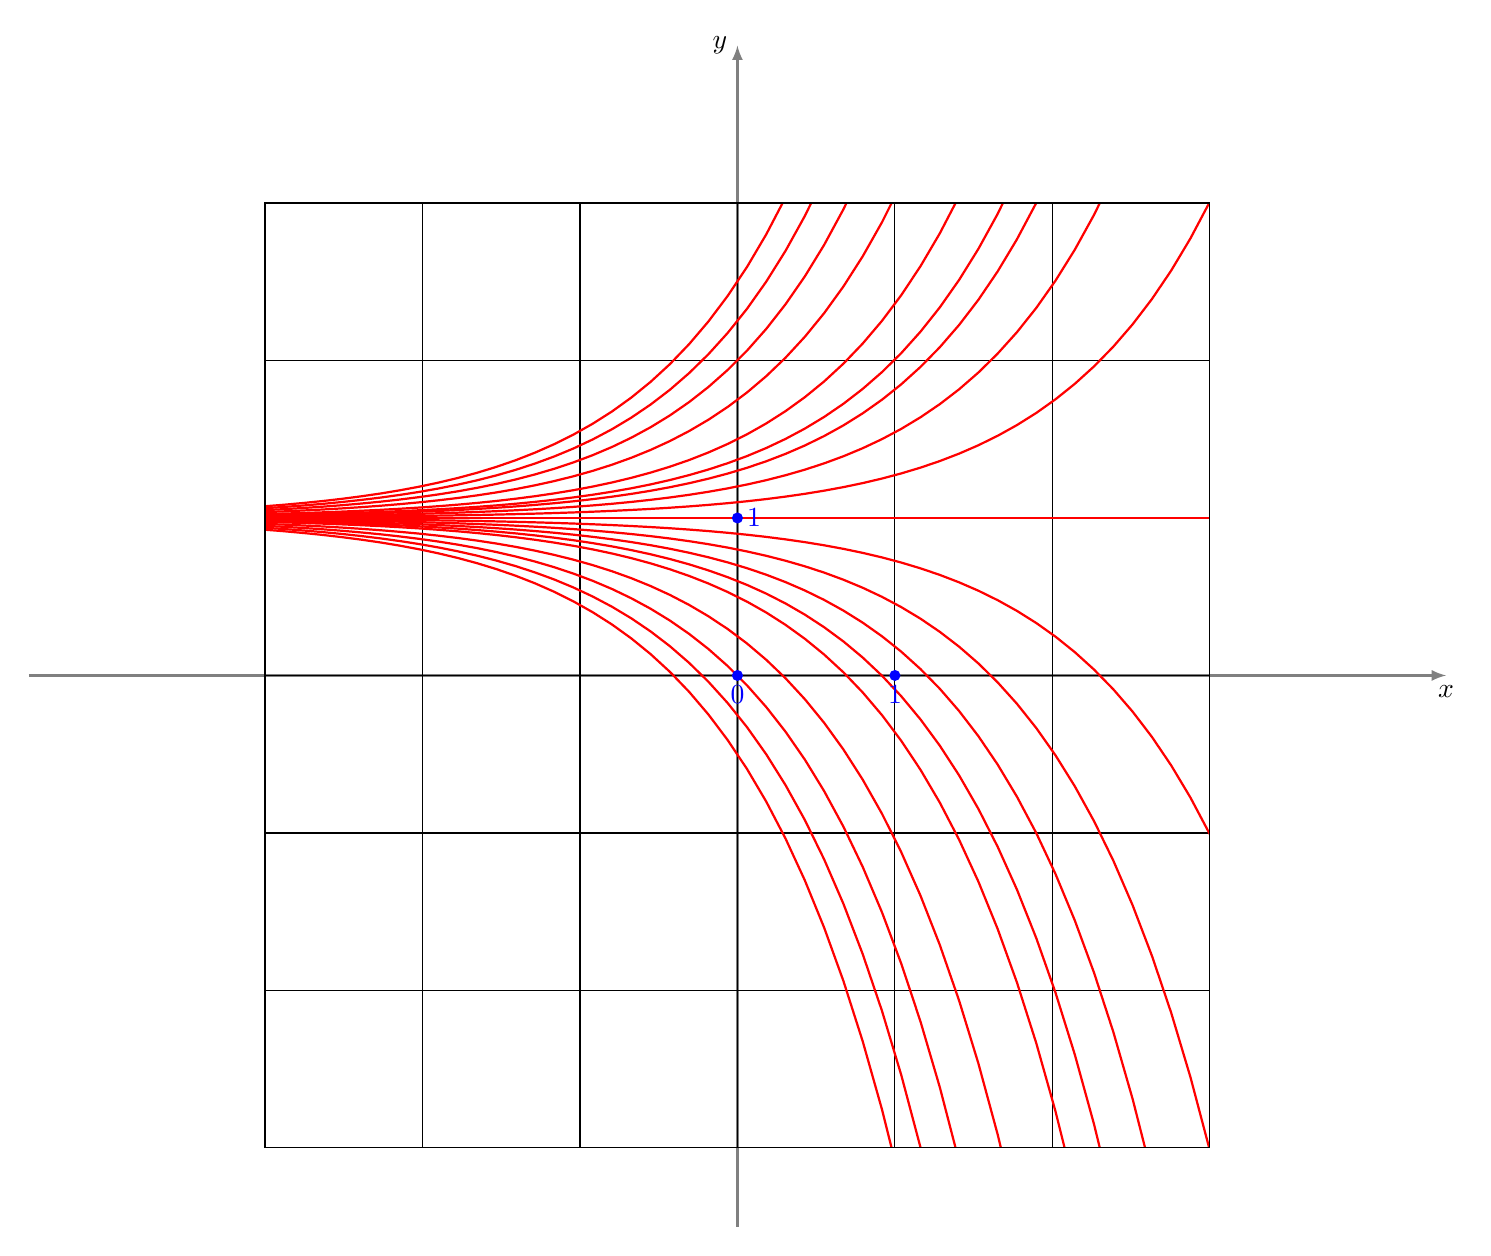
\begin{tikzpicture}[scale=2]

  \draw[->,>=latex,thick,gray] (-4.5,0) -- (4.5,0) node[below,black] {$x$};
  \draw[->,>=latex,thick,gray] (0,-3.5) -- (0,4) node[left,black] {$y$};
  \draw (-3,-3) grid (3,3);
\begin{scope}
    \clip (-3,-3) rectangle (3,3);


\foreach \k in {-1.5, -1.25,-1,-0.75,-0.5,-0.4,-0.3,-0.2,-0.1,0,0.1,0.2,0.3,0.37,0.5,0.75,1,1.25,1.5} {
  \draw[thick, color=red,domain=-3:3, samples=50] plot (\x,{\k*exp(\x)+1});
}

\end{scope}

\fill[blue] (0,0)  circle (1pt) node [below] {$0$}; 
\fill[blue] (1,0)  circle (1pt) node [below] {$1$}; 
\fill[blue] (0,1)  circle (1pt) node [right] {$1$};

\draw (-3,-3) rectangle (3,3);

\end{tikzpicture}
\end{center}


\begin{enumerate}
  \item Répondre graphiquement aux questions suivantes :
  \begin{enumerate}
    \item Quelle est la limite d'une solution en $-\infty$ ?
    \item Quelle est la solution constante ?
    \item En fonction de la valeur $f(0)$ d'une solution $f$, discuter si $f$ est croissante ou décroissante et déterminer la limite en $+\infty$.
    \item Tracer la tangente à la courbe solution qui passe par le point $(0,2)$ ; en déduire une équation approchée de cette tangente.
    \item Tracer la tangente à la courbe solution qui passe par le point $(1,-1)$ ; en déduire une équation approchée de cette tangente.
  \end{enumerate} 


  \item  Répondre par le calcul aux questions suivantes (il n'y a pas besoin de résoudre l'équation) :

  \begin{enumerate}
    \item Soit $f$ la solution dont le graphe passe par le point $(0,0)$. Combien vaut $f(0)$ ? Combien vaut $f'(0)$ ? En déduire la pente de la tangente en ce point, puis l'équation de cette tangente.

    \item  Soit $g$ la solution dont le graphe passe par le point $(1,2)$. Combien vaut $g(1)$ ? Combien vaut $g'(1)$ ? En déduire l'équation de la tangente en ce point.
  \end{enumerate} 

\end{enumerate} 
\finenonce

\indication
La pente de la tangente en $x_0$ est $f'(x_0)$.
\finindication

\correction
\sauteligne
\begin{enumerate}
  \item
  \begin{enumerate}
    \item Graphiquement on note que toutes les solutions tendent vers $1$ en $-\infty$. (Cela s'explique par le calcul, mais ce n'est pas ce qui est demandé ici.)

    \item La fonction égale à $1$ est la seule solution constante.

    \item Si $f(0)=1$, la fonction est constante égale à $1$. 
   Si $f(0)>1$, la fonction est croissante et tend vers $+\infty$ en $+\infty$.
   Si $f(0)<1$, la fonction est décroissante et tend vers $-\infty$ en $+\infty$.

    \item La tangente est tracée ci-dessous, par lecture graphique elle a pour équation $y=x+2$.

    \item La tangente est tracée ci-dessous, par lecture graphique elle a pour équation $y=-2x+1$.
  \end{enumerate} 

\begin{center}
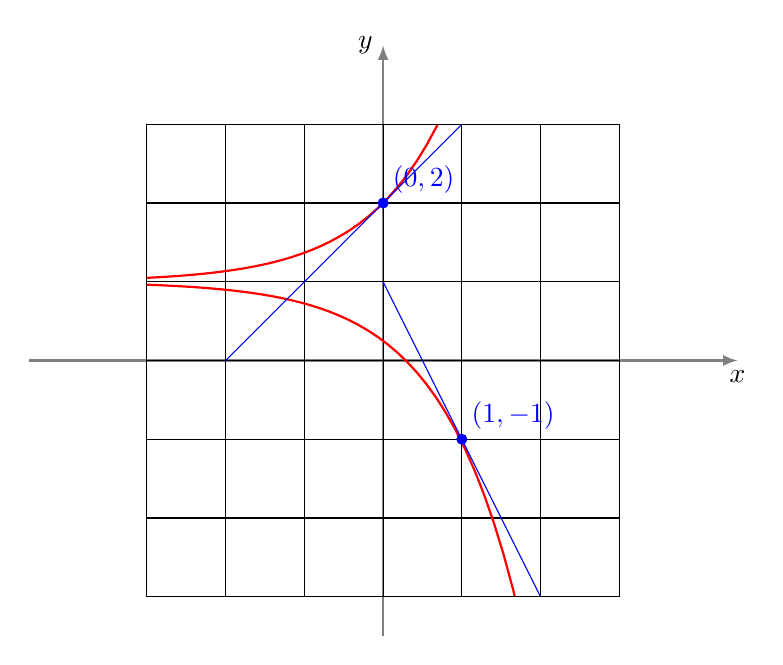
\begin{tikzpicture}[scale=1]

  \draw[->,>=latex,thick,gray] (-4.5,0) -- (4.5,0) node[below,black] {$x$};
  \draw[->,>=latex,thick,gray] (0,-3.5) -- (0,4) node[left,black] {$y$};
  \draw (-3,-3) grid (3,3);
\begin{scope}
    \clip (-3,-3) rectangle (3,3);


\foreach \k in {-0.75,1} {
  \draw[thick, color=red,domain=-3:3, samples=50] plot (\x,{\k*exp(\x)+1});
}


\fill[blue] (0,2)  circle (2pt) node[above right]{$(0,2)$};
\fill[blue] (1,-1)  circle (2pt) node[above right]{$(1,-1)$};
\end{scope}

% Tangente en (0,2)
\draw[blue] (-2,0) -- ++(3,3);

% Tangente en (1,-1)
\draw[blue] (0,1) -- ++(2,-4);

\draw (-3,-3) rectangle (3,3);

\end{tikzpicture}
\end{center}


  \item  
  \begin{enumerate}
    \item Si le graphe de $f$ passe par $(0,0)$, alors $f(0)=0$. Comme $f$ est solution de l'équation différentielle $y'=y-1$ alors pour tout $x$, $f'(x)=f(x)-1$, donc en particulier pour $x=0$ on obtient $f'(0)=f(0)-1$, donc $f'(0)=-1$.
    La pente de la tangente au graphe de $f$ en $(0,0)$ est donc $-1$. L'équation de cette tangente est donc $y=-x$ (cf graphique ci-dessous).


    \item  Si le graphe de $g$ passe par $(1,2)$, alors $g(1)=2$. Comme $g$ vérifie l'équation différentielle alors $g'(x)=g(x)-1$, donc pour $x=1$,
    $g'(1)=g(1)-1=2-1=1$. La pente de la tangente au graphe de $g$ en $(1,2)$ est donc $1$ et comme la droite passe par le point $(1,2)$, l'équation de la tangente est $y=x+1$ (cf graphique ci-dessous).
  \end{enumerate} 


\begin{center}
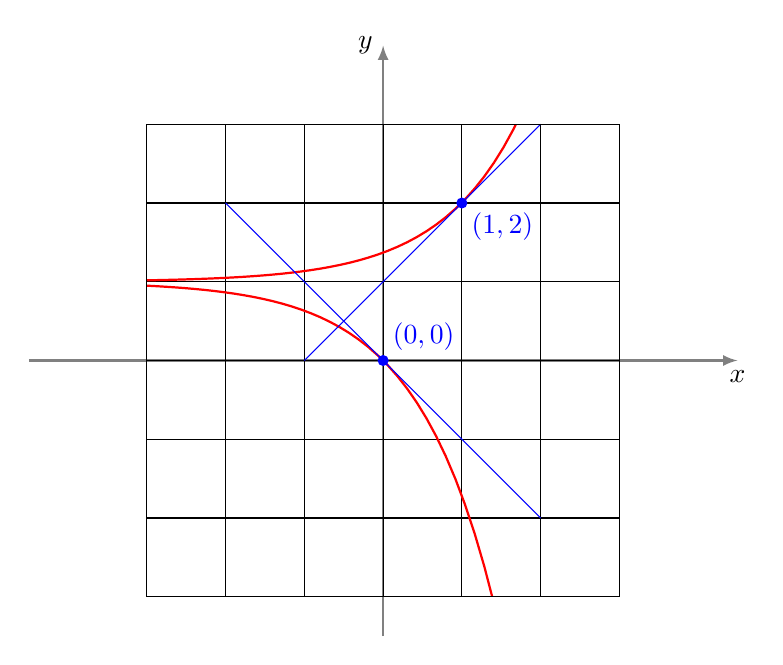
\begin{tikzpicture}[scale=1]

  \draw[->,>=latex,thick,gray] (-4.5,0) -- (4.5,0) node[below,black] {$x$};
  \draw[->,>=latex,thick,gray] (0,-3.5) -- (0,4) node[left,black] {$y$};
  \draw (-3,-3) grid (3,3);
\begin{scope}
    \clip (-3,-3) rectangle (3,3);


\foreach \k in {-1,0.37} {
  \draw[thick, color=red,domain=-3:3, samples=50] plot (\x,{\k*exp(\x)+1});
}
\fill[blue] (1,2)  circle (2pt) node[below right]{$(1,2)$}; 
\fill[blue] (0,0)  circle (2pt) node[above right]{$(0,0)$}; 

\end{scope}

% Tangente en (0,0)
\draw[blue] (-2,2) -- (2,-2);

% Tangente en (1,2)
\draw[blue] (-1,0) -- ++(3,3);

%\fill[blue] (0,0)  circle (1pt) node [below] {$0$}; 
%\fill[blue] (1,0)  circle (1pt) node [below] {$1$}; 
%\fill[blue] (0,1)  circle (1pt) node [right] {$1$};

\draw (-3,-3) rectangle (3,3);

\end{tikzpicture}
\end{center}

\end{enumerate} 
\fincorrection
\finexercice


\exercice{}
\enonce
Une tasse de café de température $T_0= 100$ degrés Celsius
est posée dans une pièce de température $T_\infty = 20$ degrés.
La loi de Newton affirme que la vitesse de décroissance de la température
est proportionnelle à l'écart entre sa température
$T(t)$ et la température ambiante $T_\infty$.

Sachant qu'au bout de $3$ minutes la température du café
est passée à $80$ degrés, quelle sera sa température au bout de $5$ minutes ?

Les questions détaillent les étapes de la résolution de ce problème :

\begin{enumerate}
  \item Justifier que la fonction température $T(t)$ satisfait l'équation différentielle 
$y' = -k(y-20)$ pour une certaine constante $k>0$.

  \item Vérifier que $T(t) = Ce^{-kt}+20$ est solution de cette équation différentielle pour toute constante $C$.

  \item Calculer $C$ en fonction de $T(0)$.

  \item Quelle est la température au bout d'un temps très long ?

  \item Déterminer la constante $k$ en utilisant que $T(3)=80$.

  \item Trouver la solution du problème.
\end{enumerate} 
\finenonce

\noindication
 
\correction
\sauteligne
\begin{enumerate}
  \item $y'$ mesure la vitesse de croissance (ou de décroissance selon le signe) de la température ; $(y-20)$ traduit l'écart entre la température du café et la température ambiante. Le coefficient $k$ exprime la proportionnalité, le signe moins venant de la décroissance de la température (le café refroidit).

  \item Pour $T(t) = Ce^{-kt}+20$, on a $T'(t) = -kCe^{-kt}$.
 Donc $-k(T(t)-20) = -k C e^{-kt} = T'(t)$ et ainsi $T(t)$ satisfait l'équation différentielle.

  \item $T(0) = Ce^{-k\cdot 0}+20 = C+20$. Comme $T(0)=100$, alors $C=80$.

  \item Comme $\lim_{t\to+\infty} Ce^{-kt} = 0$, on a $\lim_{t\to+\infty} T(t) = 20$. La température du café tendra vers $20$ degrés (c'est normal, c'est la température de la pièce).

  \item Comme $T(3)=80$ alors $80e^{-k\cdot3}+20 = 80$ donc $e^{-3k} = \frac34$.
  On compose par le logarithme des deux côtés : $\ln(e^{-3k})=\ln(\frac34)$ donc $-3k =\ln(\frac34)$ et ainsi
  $k = -\frac13\ln(\frac34) = \frac 13 \ln(\frac 43)  \simeq 0,096$. 

  \item Ainsi $T(t) \simeq 80e^{-0,096 \cdot t}+20$, donc pour $t=5$ on obtient $T(5) \simeq 80 e^{-0,096 \times 5} + 20 \simeq  69,5$ degrés Celsius.
\end{enumerate}
\fincorrection
\finexercice


%%%%%%%%%%%%%%%%%%%%%%%%%%%%%%%%%%%%%%%%%%%%%%%%%%%%%%%%%%%%
\section{$y'=ay$}

\exercice{}
\enonce
Résoudre les équations différentielles suivantes, c'est-à-dire trouver toutes les fonctions solutions.
\begin{enumerate}
  \item $y'=3y$
  \item $y'+2y=0$
  \item $4y'-5y=0$
\end{enumerate} 
\finenonce

\indication
Les solutions de $y'=ay$ sont les fonctions $y(x)=Ce^{ax}$ où $C$ est une constante.
\finindication

\correction
\sauteligne
\begin{enumerate}
  \item $y'=3y$ : les solutions sont $y(x)=Ce^{3x}$ où $C$ est une constante.
  \item $y'+2y$ équivaut à $y'=-2y$ : les solutions sont $y(x)=Ce^{-2x}$ où $C$ est une constante.
  \item $4y'-5y=0$ équivaut à $y'=\frac54y$  : les solutions sont $y(x)=Ce^{\frac54x}$ où $C$ est une constante.
\end{enumerate}
\fincorrection
\finexercice

\exercice{}
\enonce
Trouver la solution des équations différentielles suivantes vérifiant la condition initiale donnée.
\begin{enumerate}
  \item $y'=-y$ avec $y(0)=2$
  \item $y'=3y$ avec $y(0)=-1$
  \item $2y'=y$ avec $y(2)=3$
\end{enumerate} 
\finenonce

\indication
Les solutions de $y'=ay$ sont les $y(x)=Ce^{ax}$ où $C$ est une constante. 
Mais ici, il faut en plus déterminer la constante $C$ afin que $y(x_0)=y_0$ ($x_0$ et $y_0$ correspondant à la condition initiale imposée).
\finindication

\correction
\sauteligne
\begin{enumerate}
  \item $y'=-y$ : les solutions sont $y(x)=Ce^{-x}$ où $C$ est une constante.
  On veut en plus $y(0)=2$, donc $Ce^{-0}=2$, comme $e^0=1$ alors $C=2$. L'unique solution cherchée est $y(x)=2e^{-x}$.

  \item $y'=3y$ : les solutions sont $y(x)=Ce^{3x}$ où $C$ est une constante.
  On veut en plus $y(0)=-1$, donc $Ce^{3\cdot 0}=-1$, donc $C=-1$. L'unique solution cherchée est $y(x)=-e^{3x}$.

  \item $2y'=y$ : les solutions sont $y(x)=Ce^{\frac12x}$ où $C$ est une constante.
  On veut en plus $y(2)=3$, donc $Ce^{\frac12 \cdot 2}=3$, donc $C e^1=3$ d'où $C = \frac{3}{e}$. L'unique solution cherchée est $y(x)=\frac{3}{e}e^{\frac12x}$ que l'on peut écrire aussi $y(x)=3e^{\frac12x-1}$.
\end{enumerate}
\fincorrection
\finexercice


\exercice{}
\enonce
Dire si les affirmations suivantes sont vraies ou fausses. Justifier votre réponse par un résultat du cours ou un contre-exemple.
 \begin{enumerate}
  \item \og{}Les solutions de $y'=2y$ sont toutes des fonctions croissantes.\fg{}
  \item \og{}L'équation différentielle $y'=-y$ admet une seule solution constante.\fg{}
  \item \og{}Il existe une unique solution à l'équation différentielle $y'=7y$ qui vérifie $y(0)>0$.\fg{}
  \item \og{}La solution de l'équation différentielle $y'=-2y$ qui vérifie $y(0)=-1$ tend vers $-\infty$ en $+\infty$.\fg{}
\end{enumerate} 
\finenonce

\noindication

\correction
\sauteligne
 \begin{enumerate}
  \item Faux. Les solutions de $y'=2y$ sont les $y(x)=Ce^{2x}$ où $C$ est une constante réelle. Par exemple pour $C=-1$, la solution $y(x)=-e^{2x}$ est décroissante.
  \item Vrai. La seule solution constante est $y(x)=0$ (obtenue via l'expression générale $y(x) = C e^{-x}$ pour $C=0$).
  \item Faux. Il existe une solution pour chaque valeur de $C=y(0)$. Par exemple pour $C=1$, $y(x)=e^{7x}$ est solution et pour $C=2$, $y(x)=2e^{7x}$ est aussi solution.
  \item Faux. La solution cherchée est $y(x)=-e^{-2x}$ qui tend vers $0$ lorsque $x$ tend vers $+\infty$.
\end{enumerate} 
\fincorrection
\finexercice


\exercice{}
\enonce
\`A la mort d'un être vivant, le nombre $N(t)$ de noyaux radioactifs de carbone 14 (en milliards) décroît selon l'équation différentielle
$$N'(t) = -k N(t)$$
où $k>0$ est une constante.

On cherche à dater un os d'animal trouvé dans une grotte.

On prend pour temps d'origine $t=0$, la date de mort de l'animal. L'unité de temps est l'année. On sait que la \og{}demi-vie\fg{} du carbone 14 est 5500 ans, cela signifie qu'à chaque période de 5500 années, la moitié des noyaux se sont désintégrés.

On sait que le nombre de noyaux lors du vivant de l'animal était $N_0=16$ (ce nombre reste constant pour tous les animaux  vivants et commence à décroître à leur mort). On mesure $N_1 = 0,20$ le nombre de noyaux dans l'os au temps présent.
\begin{enumerate}
  \item Résoudre l'équation différentielle en fonction de $N_0$ et de $k$.
  \item La période de demi-vie donne la relation $N(5500)=\frac{N_0}{2}$. Calculer alors la valeur de la constante $k$.
  \item Combien d'années auparavant cet animal a-t-il vécu ?
\end{enumerate} 
\finenonce

\noindication

\correction
\sauteligne
\begin{enumerate}
  \item La solution de $N'(t) = -k N(t)$ est $N(t) = Ce^{-kt}$, or $N(0)=N_0=C$ donc la solution est $N(t) = N_0e^{-kt}$ autrement dit $N(t) = 16e^{-kt}$.

  \item $N(5500)=\frac{16}{2}=8$, donc $16e^{-k \cdot 5500}=8$. Cela donne $e^{-k \cdot 5500} = \frac12$. On compose par le logarithme de chaque côté : 
$\ln\big( e^{-k \cdot 5500} \big) = \ln(\frac12)$, donc $-k \cdot 5500 = -\ln(2)$. Conclusion : $k = \frac{\ln(2)}{5500} \simeq 0,000126$ et la solution est $N(t) \simeq 16 e^{-0,000126 \cdot t}$.

  \item Notons $\tau$ le temps écoulé depuis la mort de l'animal. Alors on sait que $N(\tau)=N_1$, donc $ 16 e^{-0,000126 \cdot \tau} = 0,2$. Cela donne
  $e^{-0,000126 \cdot \tau} = 0,0125$ ; donc en composant par le logarithme 
  $-0,000126 \cdot \tau = \ln(0,0125)$ ainsi $\tau \simeq 34777$. On peut donc dire que l'animal a vécu il y a environ 35 000 années. 
\end{enumerate} 
\fincorrection
\finexercice


%%%%%%%%%%%%%%%%%%%%%%%%%%%%%%%%%%%%%%%%%%%%%%%%%%%%%%%%%%%%
\section{$y'=ay+b$ et $y'=ay+f$}

\exercice{}
\enonce
Pour chacune des équations différentielles $(E)$ suivantes, 
 \begin{itemize}
  \item déterminer l'équation homogène associée,
  \item trouver les solutions $y_h(x)$ de cette équation homogène,
  \item vérifier que la fonction $y_p(x)$ est bien solution de l'équation différentielle $(E)$,
  \item en déduire toutes les solutions de $(E)$.
\end{itemize} 
 
 \begin{enumerate}
  \item $y'=-y+x^2+1$, $y_p(x)=x^2-2x+3$
  \item $y'=y+2\cos(x)$, $y_p(x)=\sin(x)-\cos(x)$ 
  \item $y'=3y+xe^{2x}$, $y_p(x)=-(x+1)e^{2x}$
\end{enumerate} 
\finenonce

\indication
Pour une équation différentielle $(E)$ : $y' = ay + f$, l'équation homogène est $y'=ay$. Si l'on note les solutions de l'équation homogène $y_h$, et une solution particulière de $(E)$ $y_p$, alors toutes les solutions de $(E)$ sont les fonctions $y_h + y_p$.
\finindication


\correction
\sauteligne
 \begin{enumerate}
  \item 
  $(E_h) : y'=-y$, $y_h(x) = Ce^{-x}$,
  $(E) : y'=-y+x^2+1$, dont $y_p(x)=x^2-2x+3$ est une solution particulière puisque $y_p'(x) = 2x-2 = -(x^2-2x+3) + x^2 + 1 = -y_p(x) + x^2 + 1$. Les solutions générales de $(E)$ sont les $y(x) = y_h(x)+y_p(x)=Ce^{-x}+x^2-2x+3$ où $C$ est une constante réelle.

  \item 
  $(E_h) : y'=y$, $y_h(x) = Ce^{x}$,
  $(E) : y'=y+2\cos(x)$, dont $y_p(x)=\sin(x)-\cos(x)$ est une solution particulière. Les solutions générales de $(E)$ sont les $y(x) = y_h(x)+y_p(x)=Ce^{x}+\sin(x)-\cos(x)$ où $C$ est une constante réelle.

  \item 
  $(E_h) : y'=3y$, $y_h(x) = Ce^{3x}$,
  $(E) : y'= 3y + x e^{2x} $, dont $y_p(x)= -(x+1)e^{2x}$ est une solution particulière. Les solutions générales de $(E)$ sont les $y(x) = y_h(x)+y_p(x)=Ce^{3x}-(x+1)e^{2x}$ où $C$ est une constante réelle.

\end{enumerate} 
\fincorrection
\finexercice

\exercice{}
\enonce
Pour chacune des équations différentielles $(E)$ suivantes, 
 \begin{itemize}
  \item déterminer l'équation homogène associée,
  \item trouver les solutions $y_h(x)$ de cette équation homogène,
  \item trouver une solution particulière $y_p(x)$ en vous aidant des indications,
  \item en déduire toutes les solutions de $(E)$.
\end{itemize} 
 
 \begin{enumerate}
  \item $y'+2y=5$, chercher une solution particulière sous la forme d'une fonction constante.  % 5
  \item $2y'-3y=e^{-x}$, chercher une solution particulière sous la forme $ke^{-x}$ où $k$ est une constante à déterminer. % -1/5e^{-x}$
  \item $y'=y + x^2$, chercher une solution particulière sous la forme $ax^2+bx+c$.    % - x^2 - 2 x - 2
\end{enumerate} 
\finenonce

\indication
Pour une équation différentielle $(E)$ : $y' = ay + f$, l'équation homogène est $y'=ay$. Si l'on note les solutions de l'équation homogène $y_h$, et une solution particulière de $(E)$ $y_p$, alors toutes les solutions de $(E)$ sont les fonctions $y_h + y_p$.
\finindication

\correction
\sauteligne
 \begin{enumerate}
  \item 
  Équation homogène : $y' + 2y = 0$ soit $y' = -2y$.\\
  Solutions de l'équation homogène : $y_h(x) = Ce^{-2x}$.\\
  Solution particulière constante : $y_p(x)= \frac 5 2$.\\ 
  Solutions générales : $y(x) = y_h(x) + y_p(x) = Ce^{-2x} + \frac 5 2$ où $C$ est une constante réelle.

  \item 
  Équation homogène : $2y'-3y = 0$ soit $y' = \frac 32 y$.\\
  Solutions de l'équation homogène : $y_h(x) = Ce^{\frac32x}$.\\
  Solution particulière : $y_p(x) = -\frac15 e^{-x}$.\\ 
  Solutions générales : $y(x) = y_h(x) + y_p(x) = Ce^{\frac32x}-\frac15 e^{-x}$ où $C$ est une constante réelle.

  \item 
  Équation homogène : $y' = y$.\\
  Solutions de l'équation homogène ; $y_h(x) = Ce^{x}$.\\
  Solution particulière : $y_p(x) = - x^2 - 2 x - 2$.\\ 
  Solutions générales : $y(x) = y_h(x) + y_p(x) = Ce^{x} - x^2 - 2 x - 2$ où $C$ est une constante réelle.
\end{enumerate} 
\fincorrection
\finexercice




\exercice{}
\enonce

Le dessin représente quelques solutions de l'équation différentielle $(E) : y'=2y+x^2e^x$.

\begin{center}
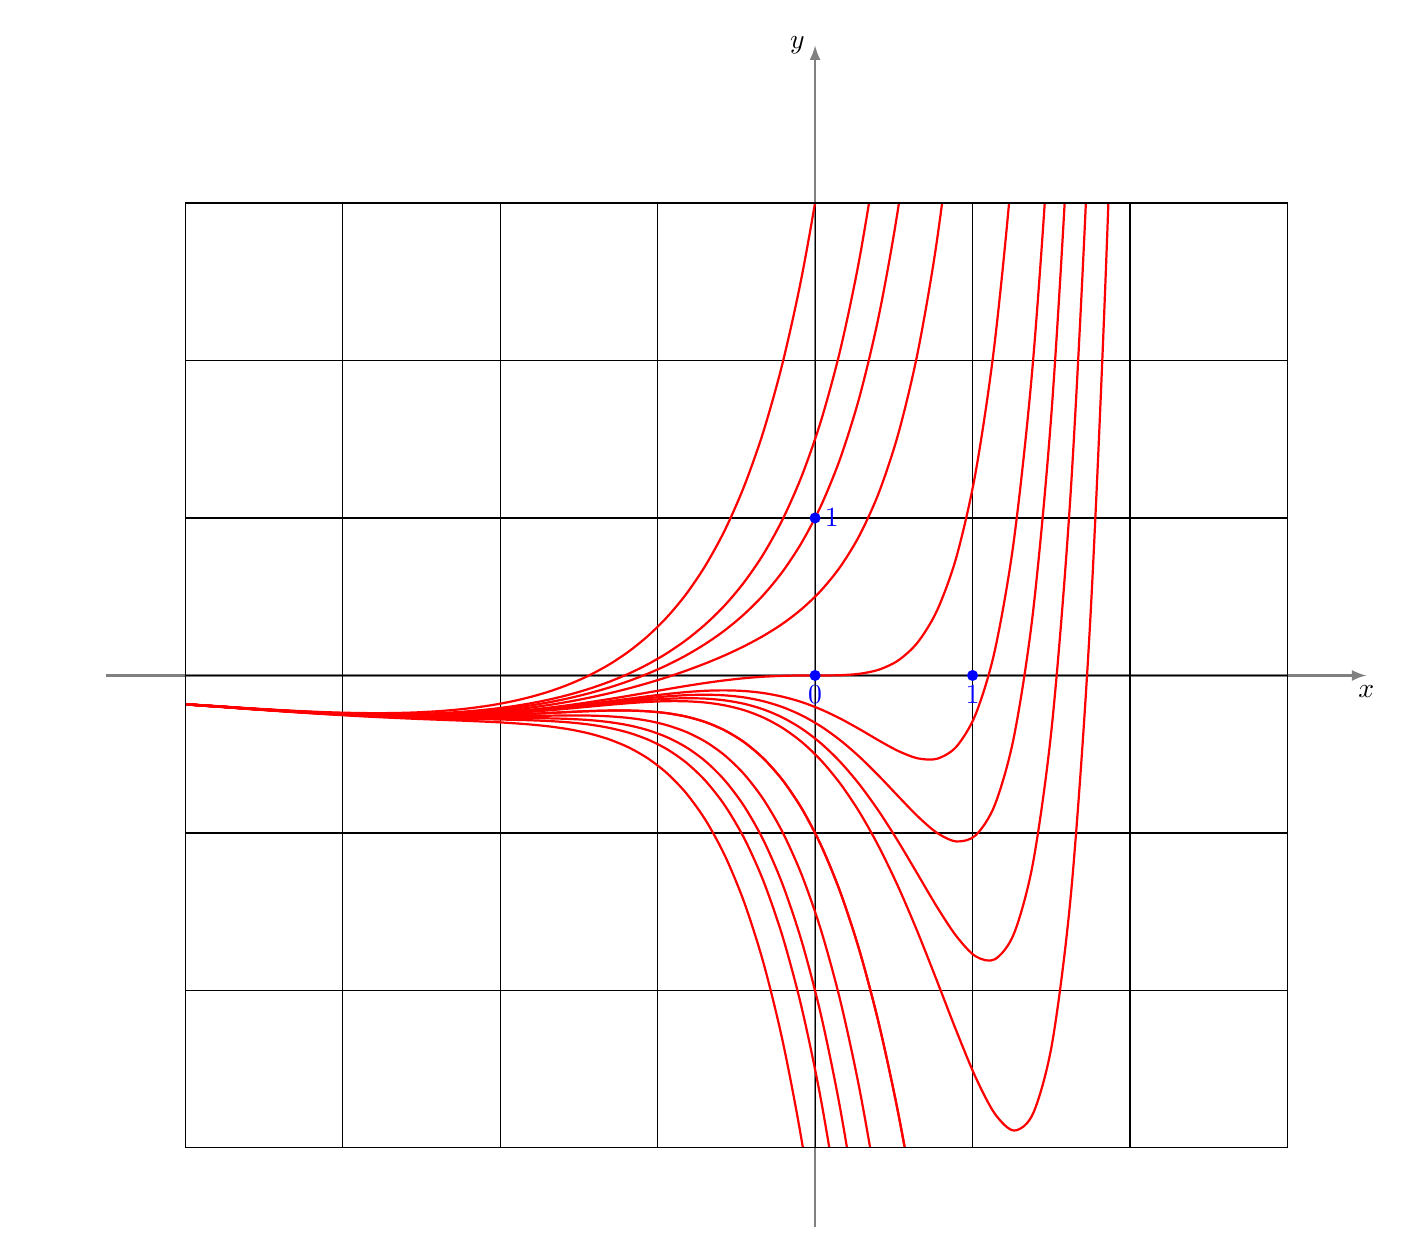
\begin{tikzpicture}[scale=2]

  \draw[->,>=latex,thick,gray] (-4.5,0) -- (3.5,0) node[below,black] {$x$};
  \draw[->,>=latex,thick,gray] (0,-3.5) -- (0,4) node[left,black] {$y$};
  \draw (-4,-3) grid (3,3);
\begin{scope}
    \clip (-5,-3) rectangle (3,3);


\foreach \k in {-1.5,-0.5,0,1,0.5,1,1.5,1.6,1.7,1.8,2,2.5,3,3.5,5} {
  \draw[thick, color=red,domain=-4:2, smooth, samples=50] plot (\x,{\k*exp(2*\x)-((\x)^2+2*\x+2)*exp(\x)}); 
}

\end{scope}

\fill[blue] (0,0)  circle (1pt) node [below] {$0$}; 
\fill[blue] (1,0)  circle (1pt) node [below] {$1$}; 
\fill[blue] (0,1)  circle (1pt) node [right] {$1$};

\draw (-4,-3) rectangle (3,3);

\end{tikzpicture}
\end{center}


\begin{enumerate}
  \item Tracer la tangente à la courbe solution qui passe par le point $(0,0)$. Retrouver son équation par le calcul  grâce à l'équation différentielle.

  \item Tracer la tangente à la courbe solution qui passe par le point $(0,1)$. Retrouver son équation par le calcul grâce à l'équation différentielle.

  \item Tracer la tangente à la courbe solution qui passe par le point $(1,-1)$. Retrouver son équation par le calcul grâce à l'équation différentielle.

  \item Déterminer les solutions $y_h(x)$ de l'équation homogène.

  \item Déterminer une solution particulière $y_p(x)$ sous la forme $(ax^2+bx+c)e^x$.

  \item En déduire toutes les solutions de $(E)$.

\end{enumerate} 
\finenonce

\noindication

\correction
\sauteligne
\begin{enumerate}
  \item Par lecture graphique il semble que la tangente en $(0,0)$ soit horizontale. Vérifions-le par le calcul. La solution $f$ dont le graphe passe par $(0,0)$ vérifie $f(0)=0$. Comme $f$ vérifie l'équation différentielle $y'=2y+x^2e^x$, alors $f'(0)=2f(0)+0^2\cdot e^0=0$, donc la tangente est bien horizontale. Son équation est $y=0$.

  \item La solution $g$ dont le graphe passe par $(0,1)$ vérifie $g(0)=1$. Comme $g$ vérifie l'équation différentielle alors $g'(0)=2g(0)+0^2\cdot e^0=2$, donc la pente de la tangente est $2$ et son équation est $y=2x+1$.

  \item La solution $h$ dont le graphe passe par $(1,-1)$ vérifie $h(1)=-1$. Comme $h$ vérifie l'équation différentielle alors $h'(1)=2h(1)+1^2\cdot e^1=e-2$, donc la pente de la tangente est $e-2$ et comme cette droite passe par $(1,-1)$ son équation est $y=(e-2)(x-1)-1$, c'est-à-dire $y=(e-2)x+1-e$.

  \item L'équation homogène est $(E_h) : y'=2y$, dont les solutions sont $y_h(x) = Ce^{2x}$, pour toute constante réelle $C$.

  \item Cherchons une solution particulière sous la forme $y_p(x) = (ax^2+bx+c)e^x$. Alors $y'_p(x) = (ax^2+(2a+b)x+b+c)e^x$.
  \begin{align*}
        & y_p(x) \text{ solution de } (E) \\
   \iff & y_p'(x) =2y_p(x) +x^2e^x  \text{ pour tout } x \in \Rr \\
   \iff & (ax^2+(2a+b)x+b+c)e^x =2(ax^2+bx+c)e^x +x^2e^x \\
   \iff & e^x\big((a+1)x^2 + (b-2a)x + (c-b) \big)  = 0 \\
   \iff & (a+1)x^2 + (b-2a)x + (c-b)  = 0 \qquad \text{car } e^x \neq 0 \\
   \iff & a+1 = 0 \quad \text{ et } \quad b-2a = 0 \quad \text{ et } \quad c-b = 0 \\
   \iff & a=-1, b=-2, c=-2 \\
  \end{align*}
   Ainsi $y_p(x) =  (-x^2 - 2x - 2)e^x = -(x^2+2x+2)e^x$ est une solution particulière.

  \item Les solutions générales de $(E)$ sont $y(x) = y_h(x) + y_p(x) = Ce^{2x} - (x^2 + 2 x + 2)e^x$ où $C$ est une constante réelle.
\end{enumerate} 
\fincorrection
\finexercice


%\exercice{}
%\enonce
% \begin{enumerate}
%  \item 
%  \item 
%  \item 
%  \item 
%\end{enumerate} 
%\finenonce
%
%\indication
%\finindication
%
%\correction
%
%\fincorrection
%\finexercice

%
%\exercice{}
%\enonce
% \begin{enumerate}
%  \item 
%  \item 
%  \item 
%  \item 
%\end{enumerate} 
%\finenonce
%
%\indication
%\finindication
%
%\correction
%
%\fincorrection
%\finexercice

\end{document}
